ابتدا برای شکل زنجیره مارکوف سکه توصیف شده خواهیم داشت:
\begin{figure}[h]
    \centering
    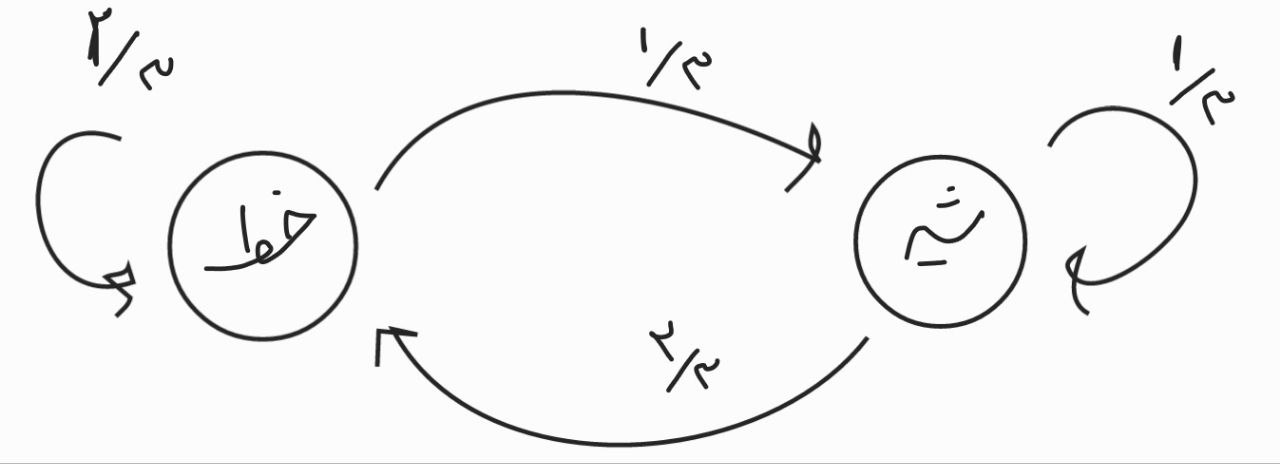
\includegraphics[scale = 0.3]{"commons/third.jpg"}
    \caption{زنجیره مارکوف برای سکه مفروض}
\end{figure}
حال برای آنکه توالی خط - شیر - خط را به دست آوریم کافی است برای اساس زنجیره مارکوف این سکه را بررسی کنیم.

می‌دانیم برای شروع با احتمال
$\frac{1}{3}$
در همان حالت می‌مانیم و با احتمال
$\frac{2}{3}$
به حالت خط برویم پس از آن یا با احتمال
$\frac{1}{3}$
در این استیت باقی می‌مانیم یا با احتمال
$\frac{2}{3}$
به حالت خط - شیر می‌رویم در اینجا نیز با احتمال
$\frac{2}{3}$
به حالت مطلوب رسیده و با احتمال
$\frac{1}{3}$
به استیت شروع می‌رویم. به این ترتیب برای امید ریاضی آن خواهیم داشت:
$$P_0 = \frac{1}{3}(P_0 + 1) + \frac{2}{3}(P_1 + 1)$$
$$P_1 = \frac{2}{3}(P_1 + 1) + \frac{1}{3}(P_2 + 1)$$
$$P_2 = \frac{2}{3} + \frac{1}{3} (P_0 + 1)$$
$$\implies P_0 = \frac{33}{4}, P_1 = \frac{27}{4}, P_2 = \frac{15}{4}$$
بنابراین امید ریاضی تعداد پرتاپ‌ها
$\frac{33}{4}$
خواهد بود.